\documentclass{standalone}
\usepackage{tikz}
\usepackage{pgfplots}
\pgfplotsset{compat=1.18}
\begin{document}
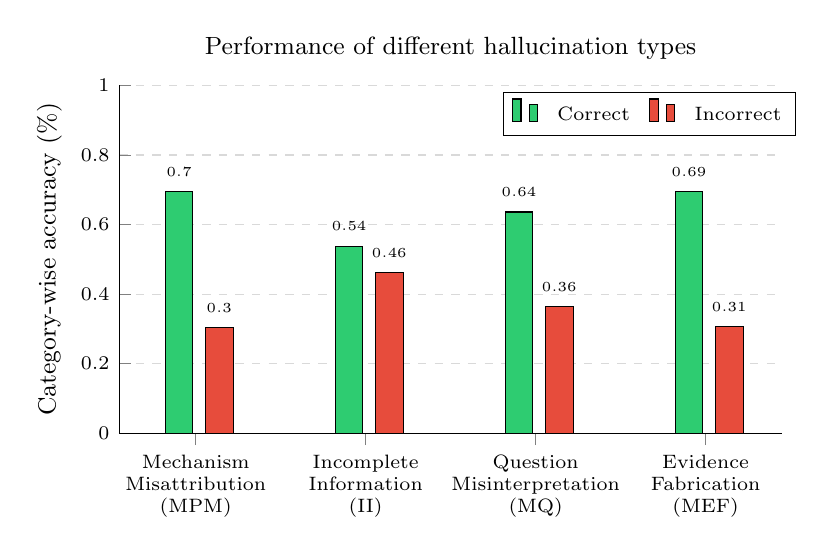
\begin{tikzpicture}[font=\small]
    % Define common colors
    \definecolor{easycolor}{RGB}{46,204,113}
    \definecolor{mediumcolor}{RGB}{52,152,219}
    \definecolor{hardcolor}{RGB}{231,76,60}
    \definecolor{correctcolor}{RGB}{46,204,113}
    \definecolor{incorrectcolor}{RGB}{231,76,60}
    
    \begin{axis}[
        at={(0,-2cm)},
        anchor=north west,
        width=10cm,
        height=6cm,
        ybar,
        bar width=10pt,
        ymin=0, ymax=1,
        ylabel={Category-wise accuracy (\%)},
        symbolic x coords={MPM, II, MQ, MEF},
        xtick=data,
        xticklabels={
            {Mechanism\\Misattribution\\(MPM)},
            {Incomplete\\Information\\(II)},
            {Question\\Misinterpretation\\(MQ)},
            {Evidence\\Fabrication\\(MEF)}
        },
        x tick label style={align=center, font=\scriptsize},
        y tick label style={font=\scriptsize},
        legend style={
            at={(0.8,0.98)}, 
            anchor=north, 
            font=\scriptsize, 
            legend columns=-1,
            transpose legend,
            row sep=0pt,
            column sep=5pt
        },
        title={Performance of different hallucination types},
        title style={font=\small},
        ymajorgrids=true,
        grid style={dashed, gray!30},
        nodes near coords,
        every node near coord/.append style={
            anchor=south,
            font=\tiny,
            yshift=2pt
        },
        enlarge x limits=0.15,
        axis lines*=left  % This removes the box and keeps only left axes
    ]
        \addplot[fill=correctcolor] coordinates {
            (MPM, 0.6953) (II, 0.5376) (MQ, 0.6361) (MEF, 0.6939)
        };
        \addplot[fill=incorrectcolor, bar shift=0.3cm] coordinates {
            (MPM, 0.3047) (II, 0.4624) (MQ, 0.3639) (MEF, 0.3061)
        };
        \legend{Correct, Incorrect}
    \end{axis}
\end{tikzpicture}
\end{document}